\section{Design} \label{sec:design}

In this section we discuss the details of the \gx{} Start Counter design.  The general engineering specifics pertaining to the scintillators, support structure, detector readout system and electronics are discussed.

\subsection{Overview} \label{sec:design_overview}
The Start Counter (ST) detector, seen in Fig.~\ref{fig:sttargetiso}, surrounds a 30~cm long super cooled liquid $\mathrm{H_{2}}$ target while providing $\sim 90 \%\ \mathrm{of\ 4 \pi}$ solid angle coverage relative to the target center.
	\begin{figure}[!htb]
		\centering
		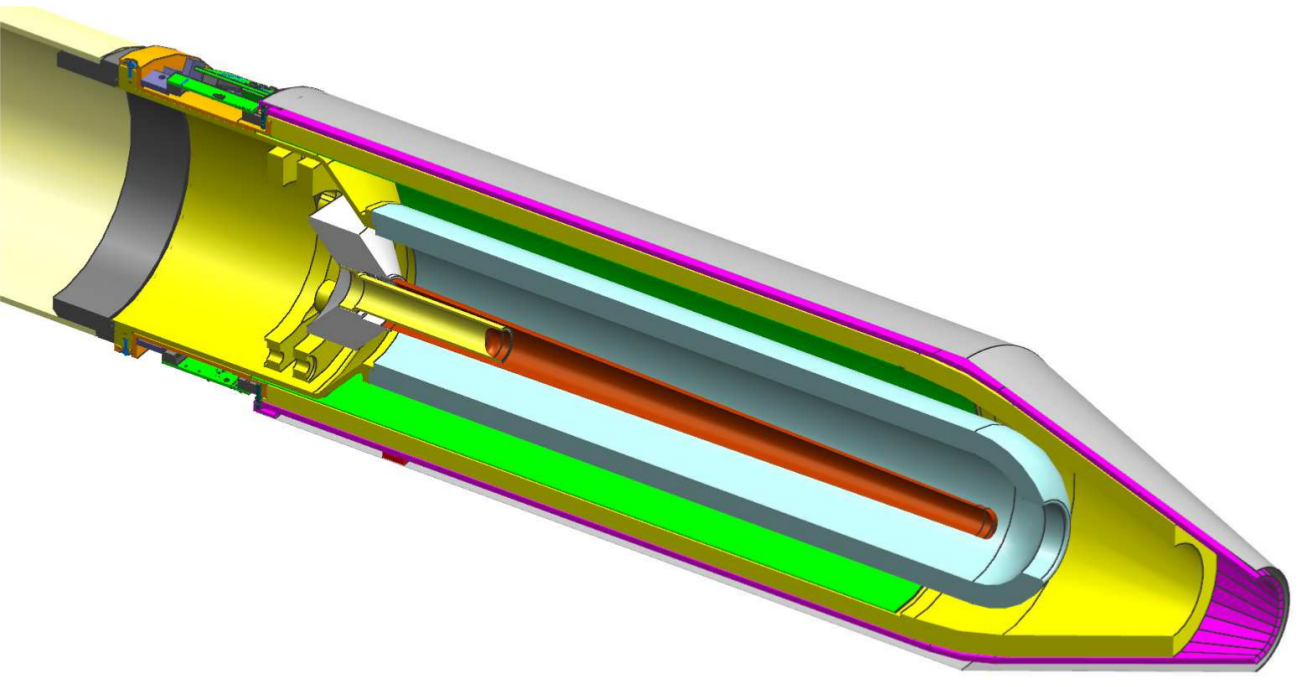
\includegraphics[width=1.0\columnwidth]{design/figs/st_target_iso}
		\caption{The \gx{} Start Counter mounted to the $\mathrm{LH_2}$ target.}
		\label{fig:sttargetiso}
	\end{figure}
The primary purpose of the ST detector is, in coincidence with the tagger, to properly identify the photon beam bucket associated with detected particles produced \textit{via} linearly polarized photons incident on the target. It is designed to operate at tagged photon intensities of up to $10^{8}\,\mathrm{\gamma/s}$ in the coherent peak.  Moreover, the ST has a high degree of segmentation for background rejection, is utilized in particle identification, and is a primary component of the level 1 trigger of the \gx{} experiment during high luminosity running\cite{pooser16}.

The ST detector consists of an array of 30 scintillators with pointed ends that bend towards the beam at the downstream end. 
	\begin{figure}[!htb]
		\centering
		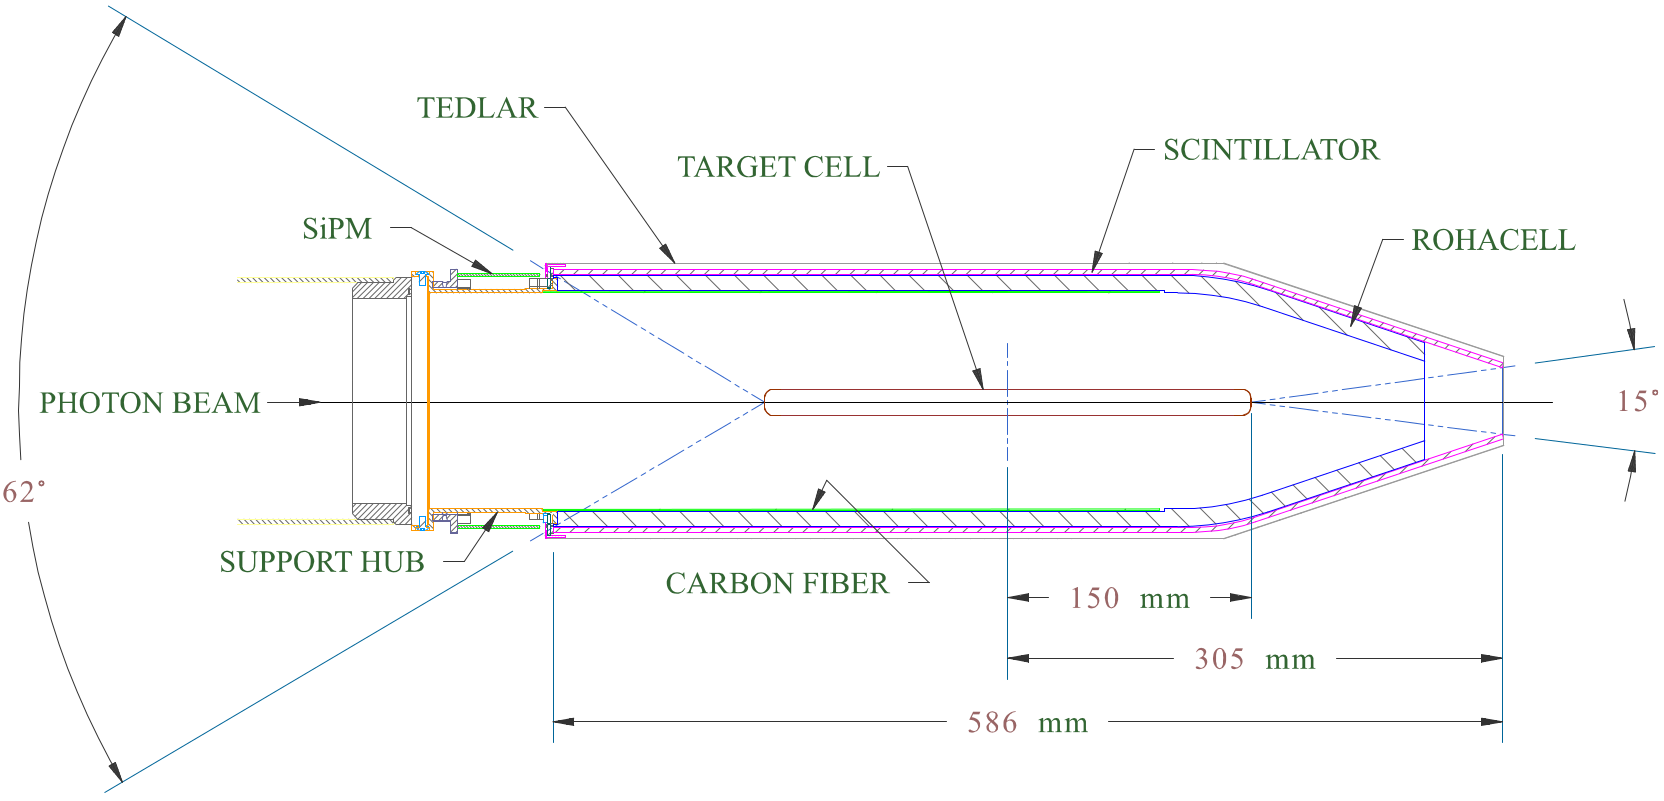
\includegraphics[width=1.0\columnwidth]{design/figs/st_2d_labels}
		\caption{Labeled 2-D cross section of the Start Counter detector.}
		\label{fig:st2dlabels}
	\end{figure}
EJ-200 scintillator material from Eljen Technology\cite{eljen}, which has a decay time of 2.1~ns and a long attenuation length\cite{ej200_specs}, was selected for this application.  The amount of support structure material was kept to an absolute minimum in the active region of the detector and is made up of low density Rohacell\cite{rohacell}. Silicon Photomultiplier (SiPM) detectors were selected as the readout system. The detectors are not affected by the high magnetic field produced by the superconducting solenoid magnet. Moreover, the SiPMs were placed as close as possible to the upstream end of each scintillator element, thereby minimizing the loss of scintillation light\cite{pooser16}.

\subsection{Scintillator Paddles} \label{sec:design_paddles}

Each individual paddle of the Start Counter was machined from a long, thin, polyvinyltoluene plastic EJ-200 scintillator bar that was diamond milled to be 600~mm in length, 3~mm thick, and $\mathrm{20 \pm 2\ mm}$ wide, by Eljen Technology.  Each scintillator was bent around a highly polished aluminum drum by applying localized infrared heating to the bend region.  The bent scintillator bars were then sent to McNeal Enterprises Inc.\cite{mcneal}, a plastic fabrication company, where they were machined to the desired geometry illustrated in Fig.~\ref{fig:stpaddleiso}.
	\begin{figure}[!htb]
		\centering
		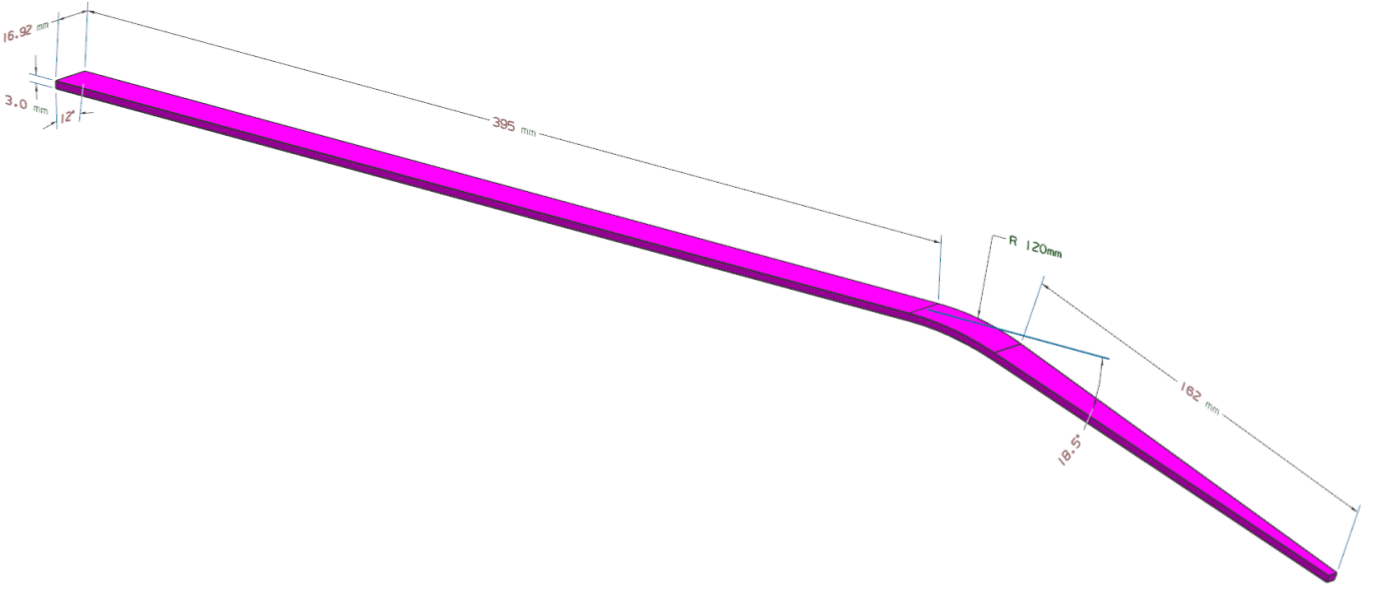
\includegraphics[width=1.0\columnwidth]{design/figs/st_paddle_iso}
		\caption{Start Counter single paddle geometry}
		\label{fig:stpaddleiso}
	\end{figure}

The paddles consist of three sections and are described from the upstream to the downstream end of the target.  The straight section is 39.5~cm in length while being oriented parallel to both the target cell and beamline..  The bend region is a $18.5^{\circ}$ arc of radius 120~cm and is downstream of the straight section. The tapered nose region is downstream of the target chamber and bends towards the beam line such that the tip of the nose is at a height of 2~cm above the beam line.  

After the straight scintillator bar was bent to the desired geometry, the two flat surfaces that are oriented orthogonal to the wide, top and bottom, surfaces were cut at a $6^{\circ}$ angle.  During this process, the width of the top and bottom surfaces were machined to be 16.92~mm and 16.29~mm wide respectively.  Thus, each of the paddles may be rotated $12^{\circ}$ with respect to the paddle that preceded it so that they form a cylindrical shape with a conical end.  This geometrical design for the ST increases solid angle coverage while minimizing multiple scattering.  

\subsection{Support Structure} \label{sec:design_support}

The ST scintillator paddles are placed atop a low density Rohacell ($\mathrm{\rho = 0.075\ g/cm^{3}}$) foam support structure which envelopes the target vacuum chamber seen in Fig.~\ref{fig:stiso}.  
	\begin{figure}[!htb]
		\centering
		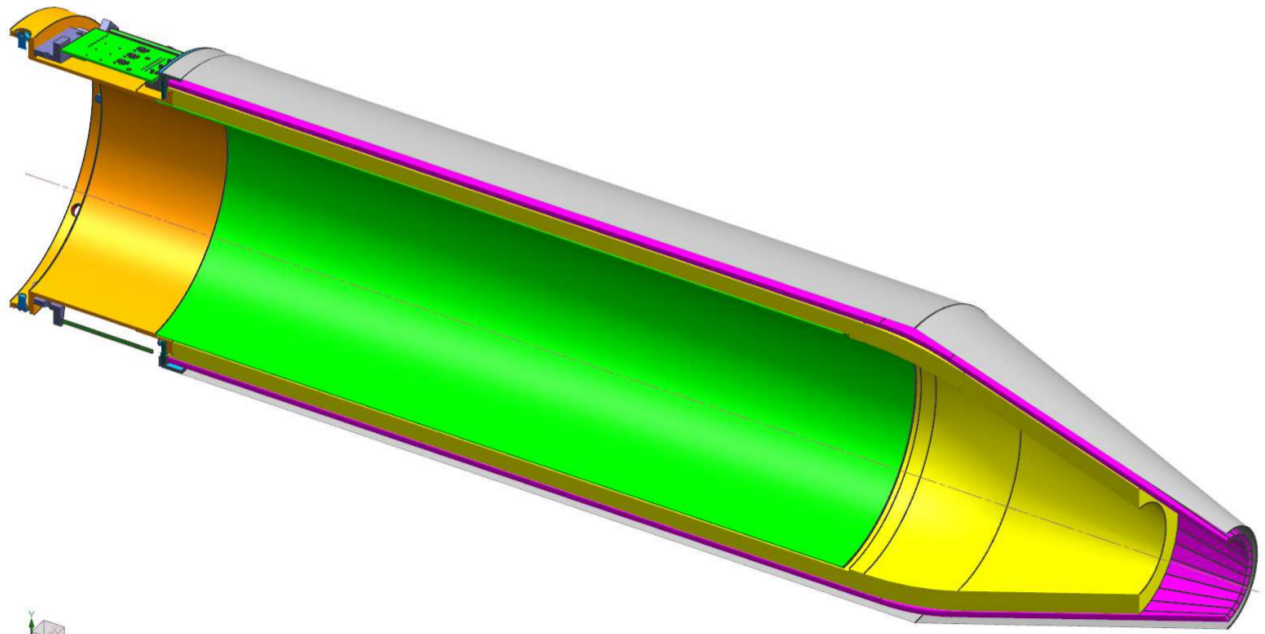
\includegraphics[width=1.0\columnwidth]{design/figs/st_iso}
		\caption{Corss section of the Start Counter support structure.}
		\label{fig:stiso}
	\end{figure}
The Rohacell, which is 11~mm thick, is rigidly attached to the upstream support chassis and extends down the length of paddles however, not to include the last few centimeters of the conical nose section.  Glued to the inner diameter of the Rohacell support structure are 3 layers of carbon fiber ($\mathrm{\rho = 1.523\ g/cm^{3}}$) each of which are $\mathrm{650\ \mu m}$ thick.  A cross section of the ST can be seen in Fig.~\ref{fig:stiso} where the carbon fiber is visible.  The carbon fiber provides additional support during the assembly process as well as long term rigidity.  

The various layers of material that comprise the ST support structure is illustrated in Fig.~\ref{fig:stmaterials}.
	\begin{figure}[!htb]
		\centering
		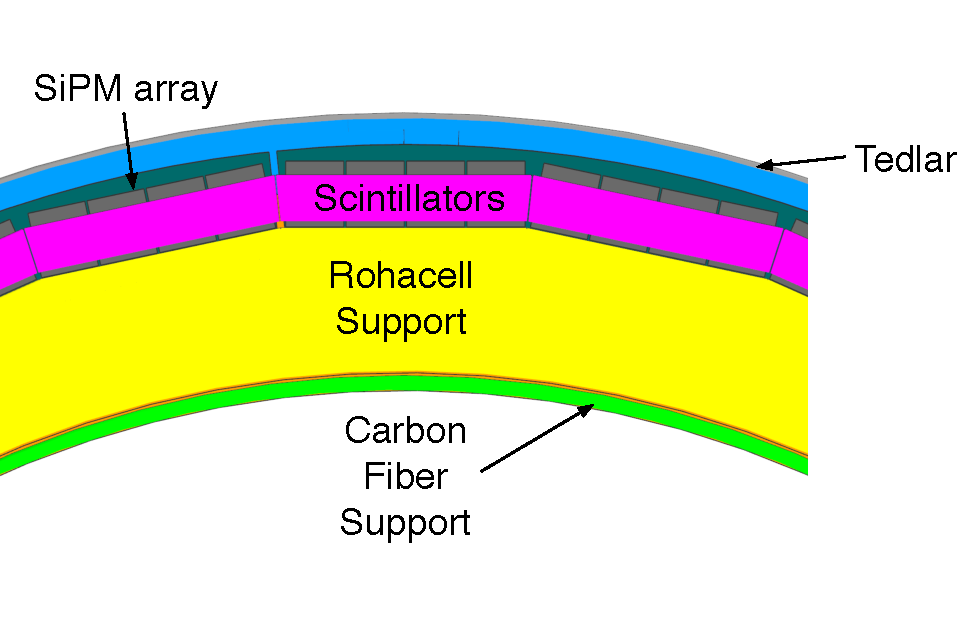
\includegraphics[width=1.0\columnwidth]{design/figs/st_materials}
		\caption{Start Counter materials.}
		\label{fig:stmaterials}
	\end{figure}
In order to ensure that the detector was light-tight, a plastic collar was placed around the top of the SiPMs at the upstream end as seen in Fig.~\ref{fig:stmaterials}.  The collar served as a lip to which a cylindrical sheet of black Tedlar was taped too.  At the tip of the nose, a cone of Tedlar was then connected to the aforementioned cylindrical section.  To make the downstream end of the ST light-tight, another cone of Tedlar was taped to the nose of the inner Rohacell support structure and then attached to the top Tedlar cone layer. 


\subsection{SiPM Readout Detectors} \label{sec:design_sipms}

The selected readout for each scintillator bar was the magnetic field insensitive Hamamatsu S10931-050P surface mounted multi-pixel photon counters (MPPCs)\cite{hamamatsu}.  An individual $\mathrm{3 \times 3\ mm^2}$ MPPC, also known as a SiPM, in the aforementioned configuration is comprised of 3600 individual, $\mathrm{50 \times 50\ \mu m^2}$, Avalanche Photo-Diode (APD) pixel counters operating in Geiger mode. The signal output from each SiPM is the total sum of the outputs from all 3600 APD pixels\cite{sipm_spec}.  The scintillation light from an individual scintillator bar is collected by an array of four of these SiPMs.

The SiPM readout detectors are housed in a ceramic case which is surface mounted to a custom fabricated printed circuit board (PCB).  The PCB is held in a fixed position while being attached to the lip of the upstream chassis \emph{via} two screws as illustrated in Fig.~\ref{fig:st1_mounted}.  The individual ST scintillators are coupled \emph{via} an air gap ($< 250 \mu m$) to groups of four SiPMs set in a circular arrangement as can be seen in Fig.~\ref{fig:st1_mounted}.
	\begin{figure}[!htb]
		\centering
		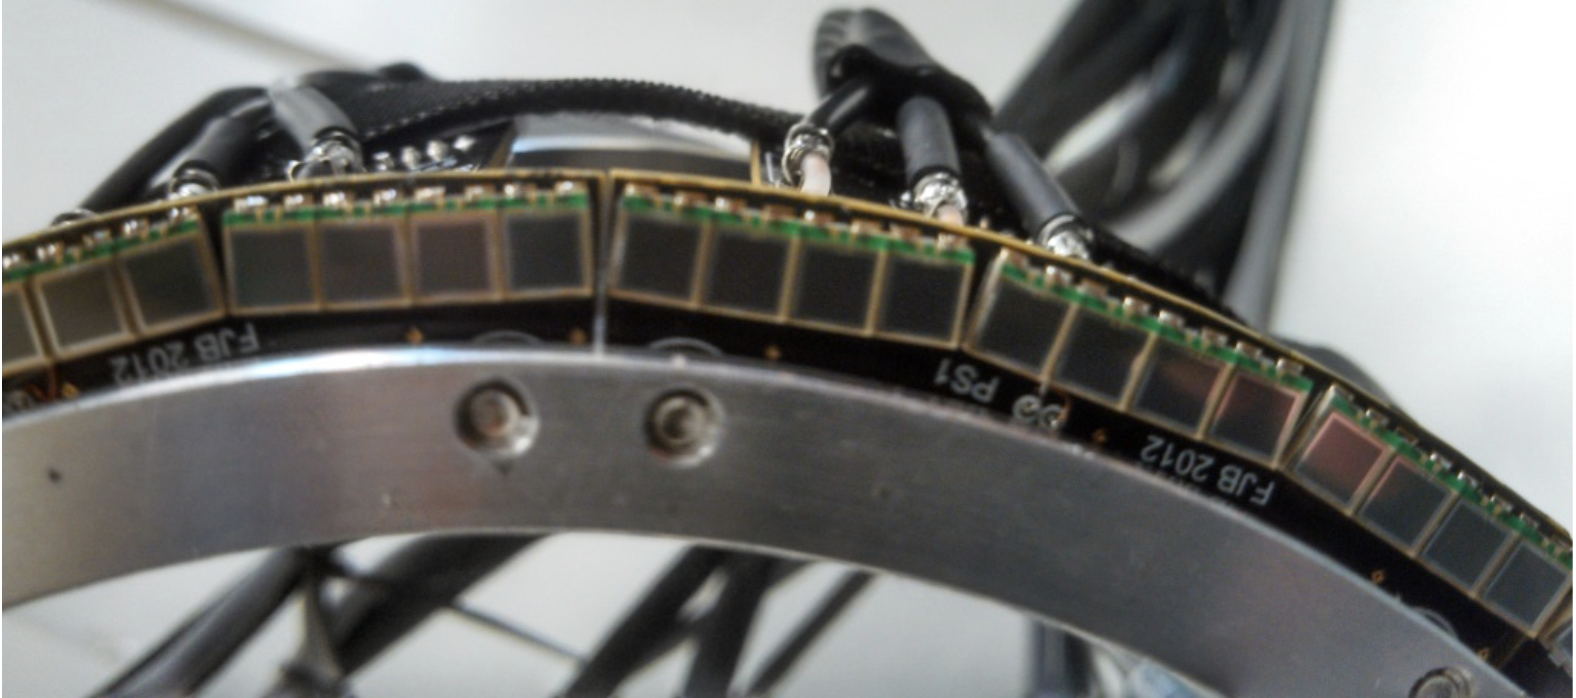
\includegraphics[width=1.0\columnwidth]{design/figs/st1_mounted}
		\caption{ST1 of Start Counter read out system. The ST1's are rigidly attached to the upstream support chassis.  Approximately 72\% of the scintillator light is collected at the upstream end.}
		\label{fig:st1_mounted}
	\end{figure}

\subsection{Readout Electronics} \label{sec:design_electronics}

The SiPMs reading out one individual paddle, are current summed prior to pre-amplification.  The output of each preamp is then split; buffered for the analog to digital converter (ADC) output, and amplified for the time to digital converter (TDC) output by a factor five relative to the ADC.  The ADC outputs are readout \emph{via} JLab VME64x 250 MHz Flash ADC modules while the TDC outputs are input into JLab leading edge discriminators, followed by a high resolution 32 channel JLab VME64x F1TDC V2 module.  Furthermore, each group of four SiPMs utilizes a thermocouple for temperature monitoring. There are 120 SiPMs in total, for a total of 30 pre-amplifier channels as seen Fig.~\ref{fig:Start Counter Electronics}.
	\begin{figure}[!htb]
		\centering
		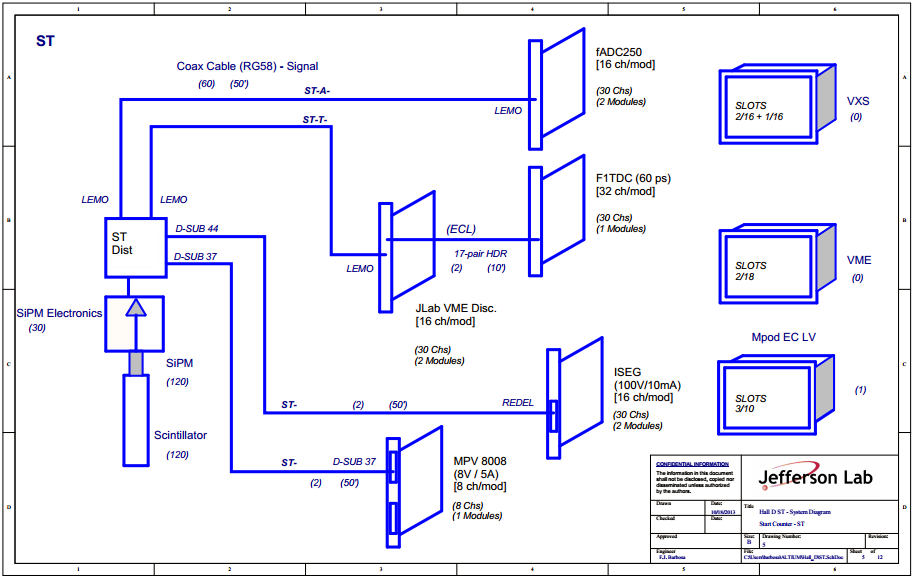
\includegraphics[width=1.0\columnwidth]{design/figs/ST_Electronics_v2}
		\caption{Start counter readout electronics diagram.}
		\label{fig:Start Counter Electronics}
	\end{figure}

There are three components that comprise the ST detector readout system.  The first component is the ST1 which holds 3 groups of 4 SiPMs as can be seen in Fig.~\ref{fig:st1_mounted}.  In order to mimic the geometry of the 30 paddle design one group of SiPM's is rotated by $12^{\circ}$ relative to the central group, while the other adjacent group is rotated by $-12^{\circ}$.  One ST1 unit will collect light from three paddles individually.  The ST1 implements the current sum and bias distribution per group of 4 SiPMs.  It also has a thermocouple for temperature monitoring.  

The second component is the ST2, seen in Fig.~\ref{fig:stfullreadout}, is a PCB that houses the signal processing electronics of the readout system.  
	\begin{figure}[!htb]
		\centering
		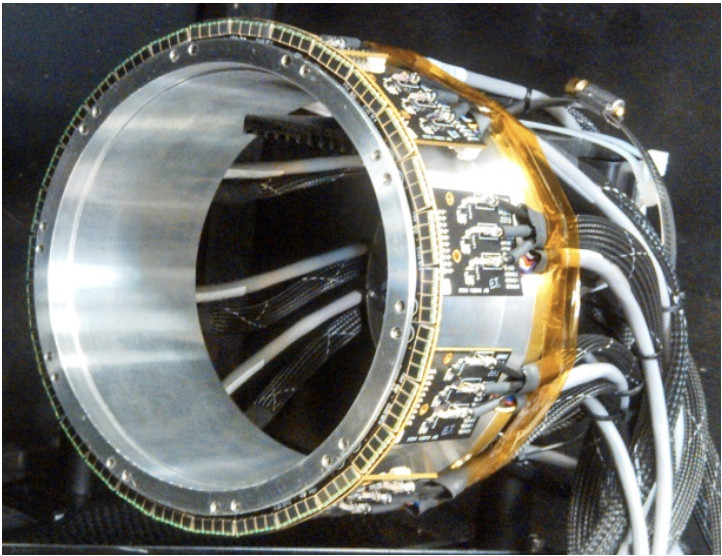
\includegraphics[width=1.0\columnwidth]{design/figs/st_full_readout}
		\caption{Fully assembled ST readout system.}
		\label{fig:stfullreadout}
	\end{figure}
It has 3 channels of pre-amplifiers, 3 buffers, and 3 factor five amplifiers.  Furthermore, it has 3 bias distribution channels with individual temperature compensation \emph{via} thermistors.  The ST2 is attached to the ST1 \emph{via} $90^{\circ}$ hermaphroditic connector.  

The third component of the readout system, the ST3 seen in Fig.~\ref{fig:st3}, provides interface to the power and bias supplies.
	\begin{figure}[!htb]
		\centering
		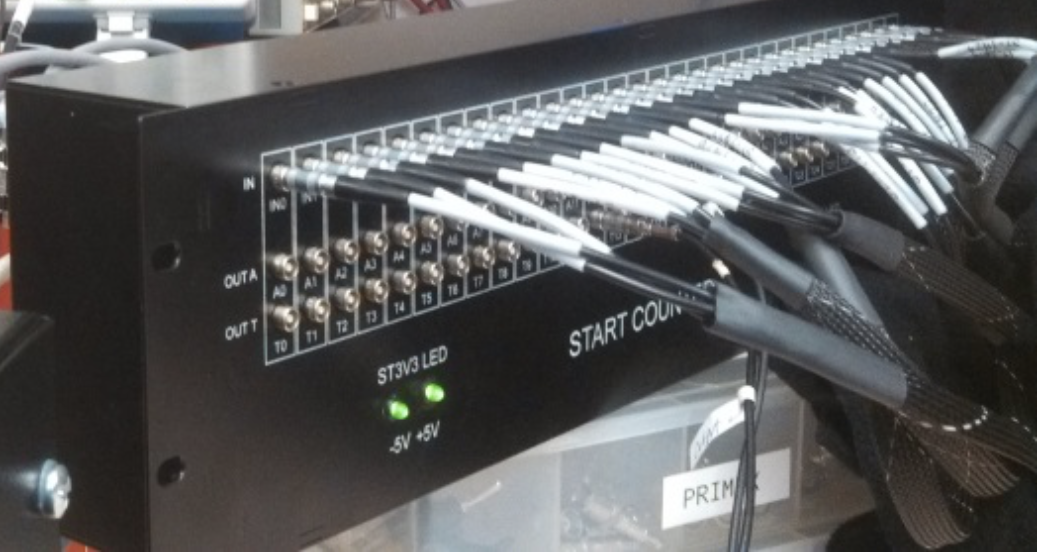
\includegraphics[width=1.0\columnwidth]{design/figs/st3}
		\caption{Start counter ST3 readout system.}
		\label{fig:st3}
	\end{figure}
It also routes the ADC and TDC outputs as well as the thermocouple output.  The ST3 connects to the ST2 \emph{via} a signal cable assembly seen in Fig.~\ref{fig:stfullreadout} and Fig.~\ref{fig:st3}.  The ST3 is installed upstream of the Start Counter and next to the beam pipe.

